\documentclass[a4paper]{article}
\usepackage[utf8]{inputenc}
\usepackage[spanish, es-tabla]{babel}

\usepackage{amsmath}
\usepackage{amsfonts}
\usepackage{amssymb}

\usepackage{float}
\usepackage{graphicx}
\graphicspath{ {./Imagenes/} }

\usepackage{multirow}
\setlength{\doublerulesep}{\arrayrulewidth}

\usepackage{array}
\newcolumntype{C}[1]{>{\centering\let\newline\\\arraybackslash\hspace{0pt}}m{#1}}

\usepackage[american]{circuitikz}

\usepackage{fancyhdr}

\usepackage{units} 

\pagestyle{fancy}
\fancyhf{}
\lhead{22.01 Teoría de Circuitos}
\rhead{Mechoulam, Lambertucci, Rodriguez, Londero}
\rfoot{Página \thepage}



\begin{document}

%%%%%%%%%%%%%%%%%%%%%%%%%%%%%%%%%%%%%%%%%%%%%%%%%%%%%%%%%%%%%%%%%%%%%%%%% 
%								CARATULA								%
%%%%%%%%%%%%%%%%%%%%%%%%%%%%%%%%%%%%%%%%%%%%%%%%%%%%%%%%%%%%%%%%%%%%%%%%% 

\begin{titlepage}
\newcommand{\HRule}{\rule{\linewidth}{0.5mm}}
\center
\mbox{\textsc{\LARGE \bfseries {Instituto Tecnológico de Buenos Aires}}}\\[1.5cm]
\textsc{\Large 22.01 Teoría de Circuitos}\\[0.5cm]


\HRule \\[0.6cm]
{ \Huge \bfseries Trabajo práctico N$^{\circ}$5}\\[0.4cm] 
\HRule \\[1.5cm]


{\large

\emph{Grupo 3}\\
\vspace{3px}

\begin{tabular}{lr} 	
\textsc{Mechoulam}, Alan  &  58438\\
\textsc{Lambertucci}, Guido Enrique  & 58009 \\
\textsc{Rodriguez Turco}, Martín Sebastian  & 56629 \\
\textsc{Londero Bonaparte}, Tomás Guillermo  & 58150 \\
\textsc{Galdeman}, Agustín & 59827\\
\end{tabular}

\vspace{20px}

\emph{Profesores}\\
Jacoby, Daniel Andrés\\
Belaustegui Goitia, Carlos\\
Iribarren, Rodrigo Iñaki\\
\vspace{3px}
%\textsc{} \\	

\vspace{100px}

\begin{tabular}{ll}

Presentado: & */*/19\\

\end{tabular}

}

\vfill

\end{titlepage}


%%%%%%%%%%%%%%%%%%%%%%%%%%%%%%%%%%%%%%%%%%%%%%%%%%%%%%%%%%%%%%%%%%%%%%%%% 
%								INFORME									%
%%%%%%%%%%%%%%%%%%%%%%%%%%%%%%%%%%%%%%%%%%%%%%%%%%%%%%%%%%%%%%%%%%%%%%%%%

\section{Introducción}

En el presente informe se estudiaron distintos tipos de filtros con un enfoque analítico teórico, práctico y además computacional. Para facilitar esto último se creó una interfaz gráfica que logra superponer distintas curvas obtenidas mediante cálculos teóricos de transferencias, mediciones con osciloscopio o simulaciones con LTSpice.

\section{Desarrollo}

\subsection{Ejercicio 1: Filtro Twin T Notch}

Se diseñó el filtro Twin T Noch mostrado en la Figura (...). Este filtro posee una frecuencia de corte de $ 8.1 \ kHz $. Para eso se seleccionó resistencias de $ 6.8 \ k\Omega $, $ 2.2 \ k\Omega $ y $ 4.7 \ k\Omega $ y capacitores de $ 4,7 \ nF $ y $ 2.2 \ nF $, considerando los valores comerciales.




\subsection{Ejercicio 2: Filtro pasa-bajos RC}
Se simuló y se armó en un protoboard un filtro pasa-bajos RC, seleccionando los valores de los componentes adecuados para lograr que la frecuencia de corte sea de $ 48 \ kHz $. Dicho circuito fue alimentado con una señal cuadrada de $ 10 \ V_{PP} $ con una frecuencia de $ 24 \ kHz $.
En forma teórica se llegó a ...
Por un lado, las simulaciones se muestran en la Figura (\ref{fig:simu2}). ...

\begin{figure}[H]
	\centering
	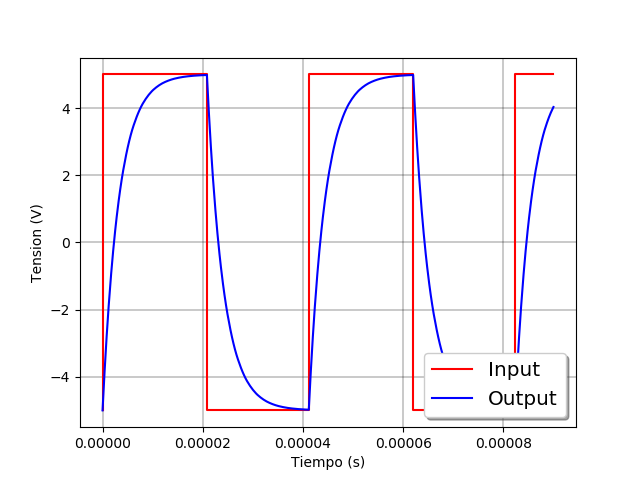
\includegraphics[width=0.9\textwidth]{Entrada-Salida.png}
\caption{Entrada (en azul) y salida (en amarillo) del circuito armado.}
	\label{fig:simu2}
\end{figure}

Por otro lado, las mediciones permitieron ver ...
Repitiendo las mediciones con una señal de las mismas características, pero con una frecuencia de $ 480 \ Hz $ se observó ...

Finalmente, se puede observar que dicho circuito puede ser utilizado como un integrador atenuado a muy altas frecuencias, ya qué

\begin{equation}
	H \left(S \right) = \frac{1}{SRC \ + 1} \approx \frac{1}{RC} \cdot \frac{1}{S}
\end{equation}

\subsection{Ejercicio 3: Plot Tool 2019}
Finalmente, en este punto se programó una GUI en Phyton que permite realizar gráficos de diagramas de BODE. Dicho programa permite analizar funciones transferencia analíticas, archivos de LTSpice, ... 
Ademas de comparar con facilidad varios diagramas de BODE y de diversas fuentes, el programa permite ...

\section{Conclusiones}


\end{document}
